\documentclass[11pt]{article}
\usepackage[margin=0.75in]{geometry}
\usepackage{graphicx}
\usepackage{parskip}
\usepackage[font=small]{caption}

\begin{document}

\section*{Barrier definitions}

For endpoint losses $C_0,C_1$ and path $\gamma(\lambda)$, the chord barrier is
the maximum excess above the straight line joining the endpoint losses,
\[
B_{\mathrm{chord}}=\max_\lambda\left[C(\gamma(\lambda))-((1-\lambda)C_0+\lambda C_1)\right].
\]
The worse-endpoint barrier is the maximum excess above the worse endpoint,
\[
B_{\mathrm{worse}}=\max_\lambda C(\gamma(\lambda))-\max(C_0,C_1).
\]

\begin{center}
    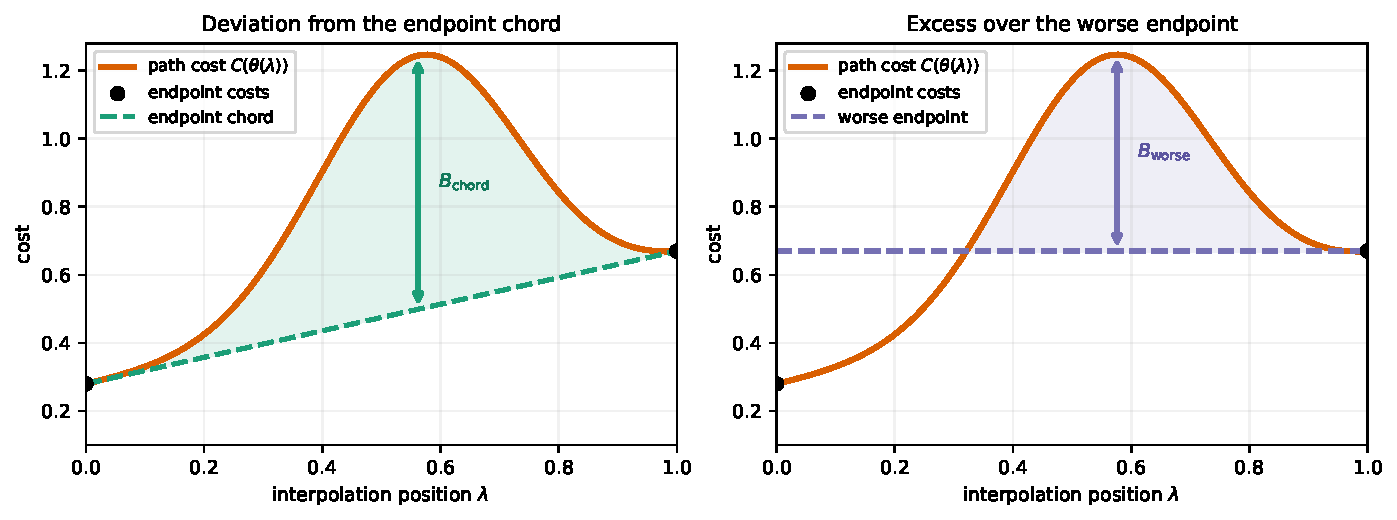
\includegraphics[width=0.78\linewidth]{../stage_connectivity_report/figures/barrier_definitions.pdf}
\end{center}

\section*{Cross-stage barrier comparison}

The figure shows the best-overall test-loss barriers for
$A_{\mathrm{final}}$--$B_n$. It compares $B_{\mathrm{chord}}$ and
$B_{\mathrm{worse}}$, with mean $\pm$ one standard deviation over three seed
pairs.

\begin{figure}[h]
    \centering
    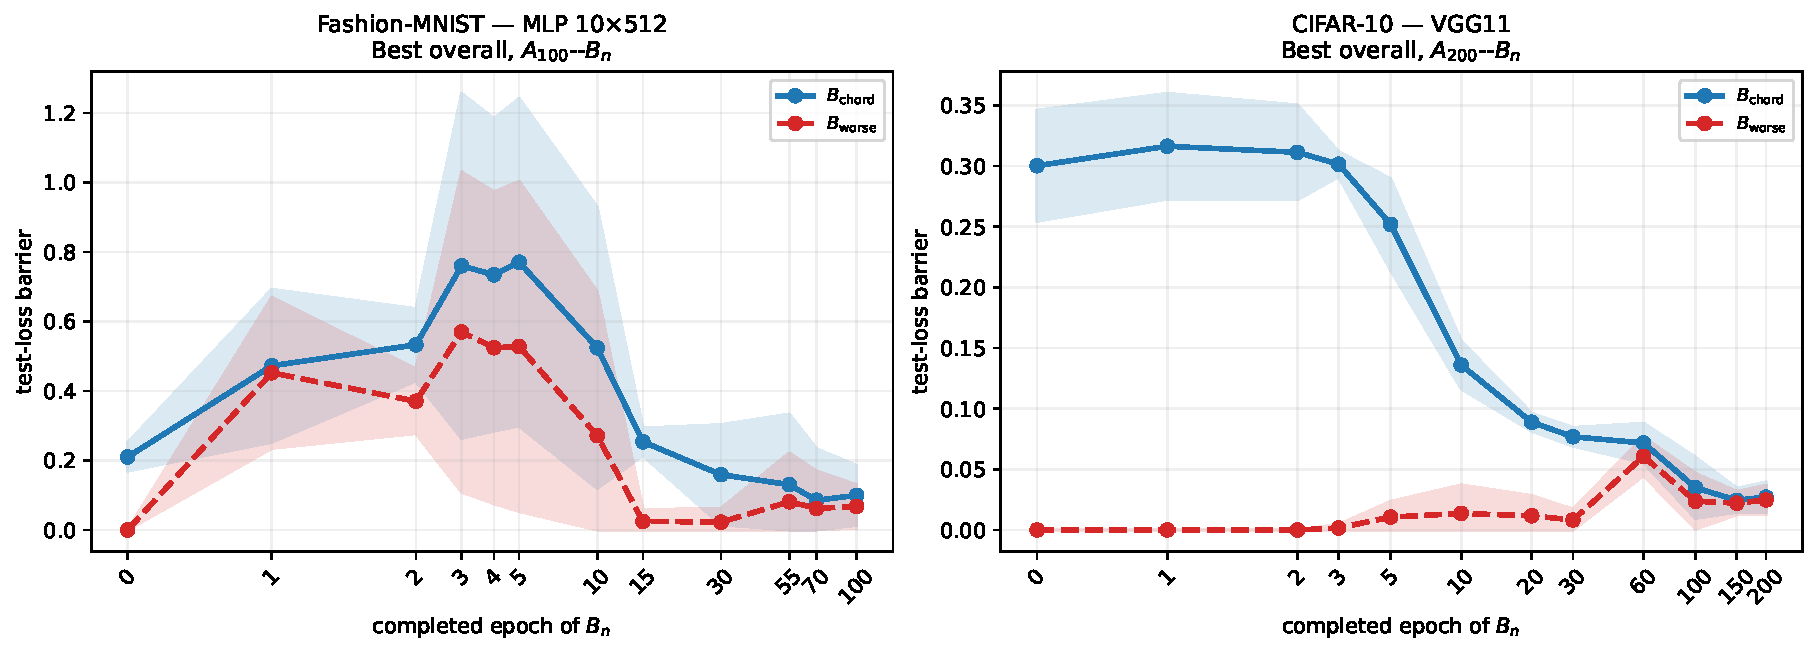
\includegraphics[width=\linewidth]{../stage_connectivity_report/figures/overall_afinal_bn_test_loss_barriers_by_architecture.pdf}
\end{figure}

The CIFAR-10/VGG11 result is the one already shown previously.  I added the
same view for the Fashion-MNIST MLP.  I am not sure what to conclude from this
comparison yet.

\end{document}
